
	\hypertarget{UC1}{}
	\subsection{Caso d'uso UC1: Configurazione Aziendale}
	
	\begin{figure}[H]
		\centering
		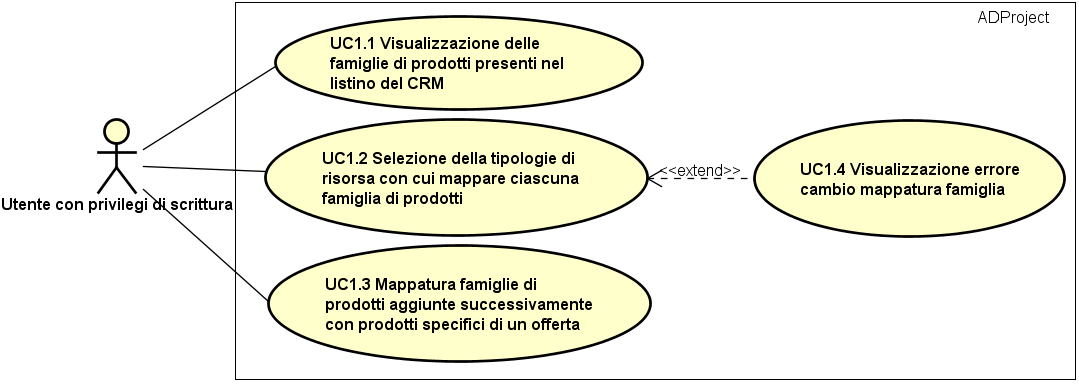
\includegraphics[scale=0.6]{images/useCase/UC1}
		\caption{Use Case 1 - Configurazione aziendale}
		%\caption{}
		\label{fig:uc1}
	\end{figure}
	\begin{longtable}{ | p{2.7cm} | p{12cm} |}
		\hline \textbf{Attori} & Utente con privilegi di scrittura\\ 
		\hline \textbf{Descrizione} & Attraverso l’interfaccia di configurazione aziendale, l’utente coi permessi corretti è in grado di visualizzare le impostazioni riguardanti la configurazione aziendale e modificarle\\ 
		\hline \textbf{Scenario Principale} & \begin{enumerate}
			\itemsep-0.5em 
			\item L’utente visualizza la lista delle famiglie di prodotti presenti nel listino del CRM  (UC1.1);
			\item L’utente seleziona la tipologia di risorse con cui andare a mappare ciascuna famiglia di prodotti  (UC1.2);
			\item L’utente mappa eventuali famiglie di prodotti non mappate o prodotti specifici di un’offerta che non sono stati mappati  (UC1.3).
			
		\end{enumerate}
		\\ 
		\hline \textbf{Postcondizione} & Sono state visualizzate ed eventualmente modificate le associazioni tra le famiglie di prodotti e le tipologie di risorse\\ 
		\hline 
	\end{longtable}
	
	\hypertarget{UC1.2}{}
	\subsection{Caso d'uso UC1.2: Selezione della tipologie di risorsa con cui mappare ciascuna famiglia di prodotti}
	
	\begin{figure}[H]
		\centering
		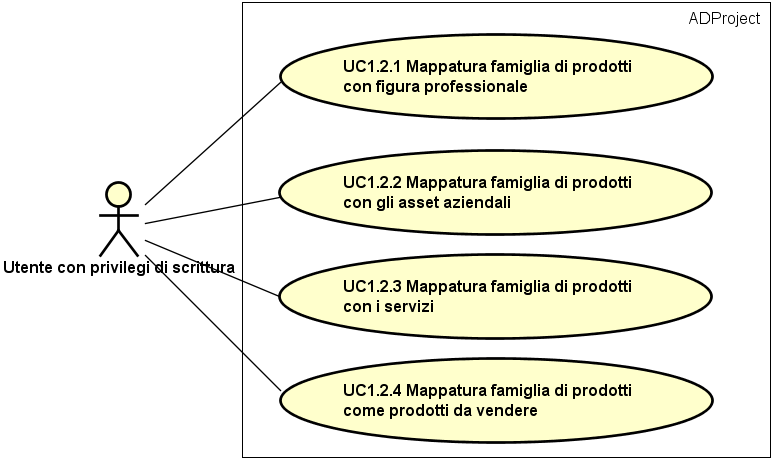
\includegraphics[width=\linewidth]{images/useCase/UC1_2}
		\caption{Use Case 1.2 - Mappatura tipologie risorse / famiglie prodotti}
		%\caption{}
		\label{fig:uc1.2}
	\end{figure}

	\begin{longtable}{ | p{2.7cm} | p{12cm} |}
		\hline \textbf{Attori} & Utente con privilegi di scrittura\\ 
		\hline \textbf{Descrizione} & Attraverso l’interfaccia di configurazione aziendale, l’utente coi permessi corretti è in grado di specificare con quale tipologia di risorsa (figura professionale, asset o servizio) dovrà essere mappata ciascuna tipologia di prodotto proveniente dal CRM\\ 
		\hline \textbf{Scenario Principale} & \begin{enumerate}
			\itemsep-0.5em 
			\item L’utente mappa una famiglia di prodotti con le figure professionali necessarie per un progetto  (UC1.2.1);
			\item L’utente mappa una famiglia di prodotti con gli asset necessarie per un progetto  (UC1.2.2);
			\item L’utente mappa una famiglia di servizi necessari per un progetto  (UC1.2.3);
			\item L’utente mappa una famiglia di prodotti come prodotti venduti (UC1.2.4).
			
		\end{enumerate}
		\\ 
		\hline \textbf{Estensioni} & \begin{enumerate}
			\item L’utente visualizza un messaggio di errore se tenta di cambiare la mappatura di una famiglia dopo che sono già stati importati prodotti relativi a quella famiglia  (UC1.4);
			
		\end{enumerate}
		\\ 
		\hline \textbf{Postcondizione} & Per almeno una famiglia di prodotto è stata modificata l’associazione ad una tipologia di risorsa. \\ 
		\hline 
	\end{longtable}
	
	\hypertarget{UC1.3}{}
	\subsection{Caso d'uso UC1.3: Mappatura famiglie di prodotti aggiunte successivamente con prodotti specifici di un offerta}
	\begin{figure}[H]
		\centering
		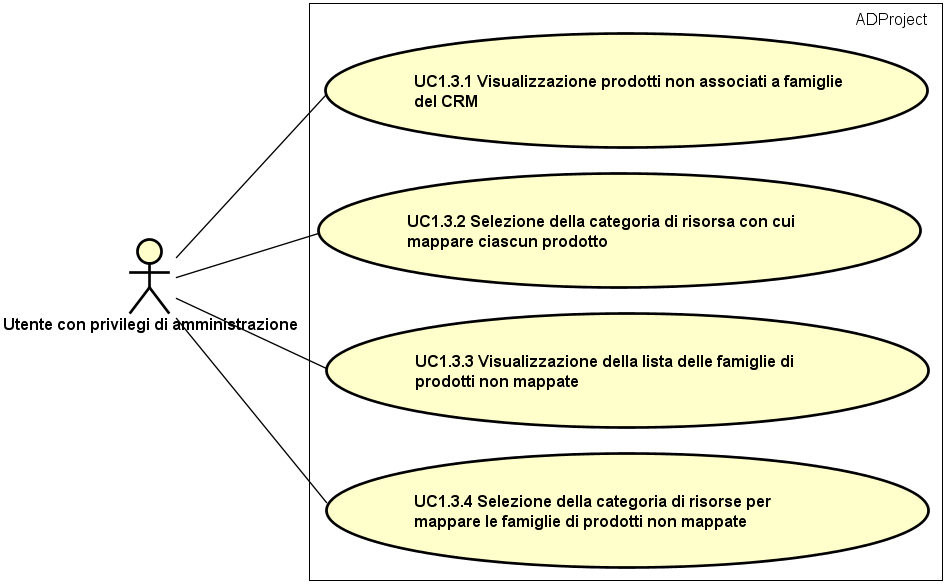
\includegraphics[scale=0.6]{images/useCase/UC1_3}
		\caption{Use Case 1.3 - Mappatura famiglie prodotti / prodotti offerta}
		%\caption{}
		\label{fig:uc1.3}
	\end{figure}
	\begin{longtable}{ | p{2.7cm} | p{12cm} |}
		\hline \textbf{Attori} & Utente con privilegi di scrittura\\ 
		\hline \textbf{Descrizione} & Attraverso l’interfaccia di configurazione di progetto, l’utente coi permessi corretti è in grado di effettuare una mappatura \textit{just-in-time} di eventuali prodotti legati all’offerta che appartengono ad una famiglia di prodotti non mappata (perché ad esempio è stata aggiunta da poco nel CRM) o che non sono associati ad una famiglia (perché magari sono prodotti associati puntualmente all’offerta\\ 
		\hline \textbf{Scenario Principale} & \begin{enumerate}
			\itemsep-0.5em 
			\item L’utente visualizza la lista dei prodotti non associati ad alcuna famiglia del CRM  (UC1.3.1);
			\item L’utente seleziona la categoria di risorsa con cui mappare ciascun prodotto  (UC1.3.2);
			\item L’utente visualizza la lista delle famiglie di prodotti non mappate  (UC1.3.3);
			\item L’utente seleziona la categoria di risorsa con cui mappare ciascuna famiglia  (UC1.3.4).
			
		\end{enumerate}
		\\ 
		\hline \textbf{Postcondizione} & Sono state potenzialmente modificate le mappature dei prodotti\\ 
		\hline 
	\end{longtable}
	
	\hypertarget{UC2}{}
	\subsection{Caso d'uso UC2: Gestione delle anagrafiche aziendali}
	\begin{figure}[H]
		\centering
		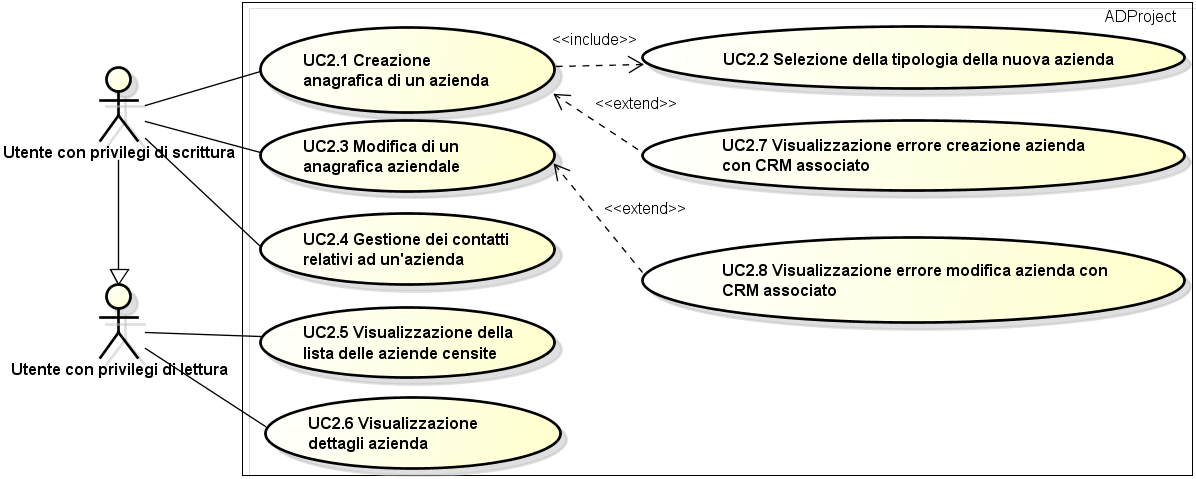
\includegraphics[scale=0.50]{images/useCase/UC2}
		\caption{Use Case 2 - Gestione anagrafiche aziendali}
		%\caption{}
		\label{fig:uc2}
	\end{figure}
	\begin{longtable}{ | p{2.7cm} | p{12cm} |}
		\hline \textbf{Attori} & Utente con privilegi di lettura, Utente con privilegi di scrittura\\ 
		\hline \textbf{Descrizione} & Attraverso l’interfaccia di gestione delle anagrafiche aziendali, l’utente coi permessi corretti è in grado di visualizzare le informazioni relative alle schede di anagrafica aziendali e modificarle\\ 
		\hline \textbf{Scenario Principale} & \begin{enumerate}
			\itemsep-0.5em 
			\item L’utente crea un’anagrafica di un’azienda  (UC2.1);
			\item L’utente modifica l’anagrafica di un’azienda già censita  (UC2.3);
			\item L’utente gestisce i contatti relativi ad un’azienda  (UC2.4);
			\item L’utente visualizza la lista delle aziende censite nel sistema  (UC2.5);
			\item L’utente visualizza i dettagli relativi ad una azienda censita nel sistema  (UC2.6).
			
		\end{enumerate}
		\\ 
		\hline \textbf{Postcondizione} & Sono state visualizzate ed eventualmente modificate le anagrafiche aziendali\\ 
		\hline 
	\end{longtable}
	
	\hypertarget{UC2.4}{}
	\subsection{Caso d'uso UC2.4: Gestione dei contatti relativi ad un'azienda}
	\begin{figure}[H]
		\centering
		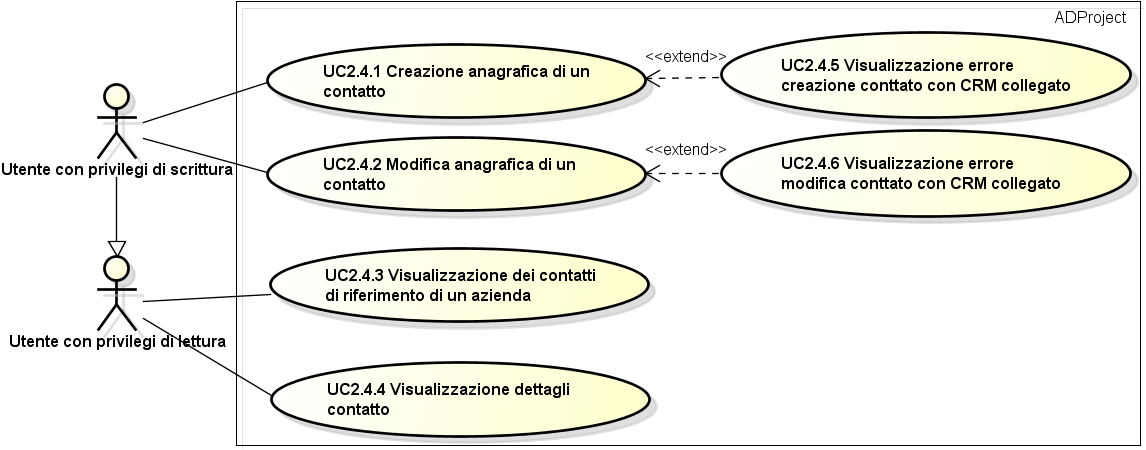
\includegraphics[scale=0.52]{images/useCase/UC2_4}
		\caption{Use Case 2.4 - Gestione contatti aziendali}
		%\caption{}
		\label{fig:uc2.4}
	\end{figure}
	\begin{longtable}{ | p{2.7cm} | p{12cm} |}
		\hline \textbf{Attori} & Utente con privilegi di scrittura\\ 
		\hline \textbf{Descrizione} & Attraverso l’interfaccia di gestione delle anagrafiche aziendali, l’utente coi permessi corretti è in grado di visualizzare le informazioni sui contatti di riferimento per le diverse aziende ed eventualmente modificarle\\ 
		\hline \textbf{Scenario Principale} & \begin{enumerate}
			\itemsep-0.5em 
			\item L’utente crea un’anagrafica di contatto ;
			\item L’utente modifica l’anagrafica di un contatto già censito ;
			\item L’utente visualizza la lista dei contatti di riferimento per una specifica azienda ;
			\item L’utente visualizza i dettagli relativi ad un contatto.
			
		\end{enumerate}
		\\ 
		\hline \textbf{Postcondizione} & Sono state visualizzate ed eventualmente modificate le informazioni relative ai contatti di riferimento per un’azienda\\ 
		\hline 
	\end{longtable}
	
	\hypertarget{UC3}{}
	\subsection{Caso d'uso UC3: Gestione dei progetti}
	\begin{figure}[H]
		\centering
		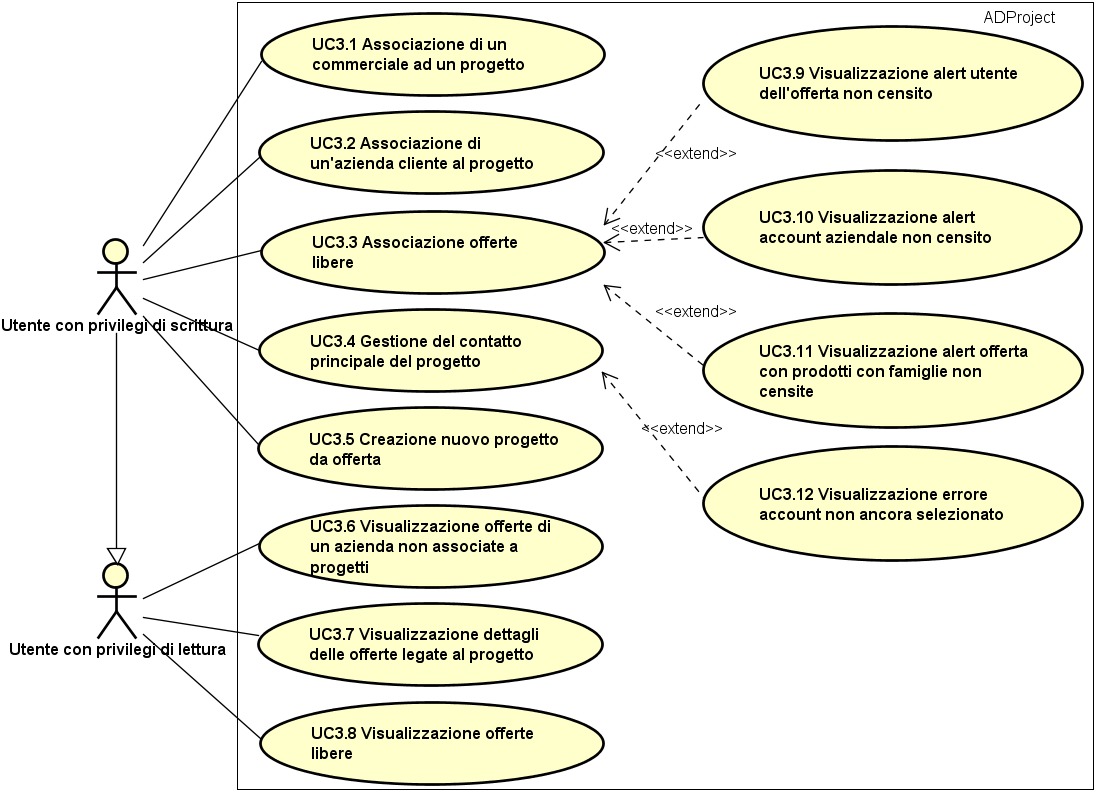
\includegraphics[scale=0.55]{images/useCase/UC3}
		\caption{Use Case 3 - Gestione progetti}
		%\caption{}
		\label{fig:uc3}
	\end{figure}
	\begin{longtable}{ | p{2.7cm} | p{12cm} |}
		\hline \textbf{Attori} & Utente con privilegi di lettura, Utente con privilegi di scrittura\\ 
		\hline \textbf{Descrizione} & Attraverso l’interfaccia di configurazione di progetto, l’utente coi permessi corretti è in grado di modificare le informazioni di progetto \\ 
		\hline \textbf{Scenario Principale} & \begin{enumerate}
			\itemsep-0.5em 
			\item L’utente associa un commerciale ad un progetto  (UC3.1);
			\item L’utente associa una delle aziende clienti censite al progetto  (UC3.2);
			\item L’utente associa una o più offerte libere al progetto selezionato  (UC3.3);
			\item L’utente gestisce il contatto principale di riferimento per un progetto  (UC3.4);
			\item L’utente visualizza la lista delle offerte libere (non associate ad alcun progetto) relative al cliente selezionato  (UC3.6);
			\item L’utente visualizza i dettagli delle offerte associate al progetto  (UC3.7);
			\item L’utente visualizza la lista di tutte le offerte libere  (UC3.8);
			\item L’utente può creare un progetto a partire da un’offerta  (UC3.5).
			
		\end{enumerate}
		\\ 
		\hline \textbf{Postcondizione} & Sono modificate le informazioni relative ad un progetto. \\ 
		\hline 
	\end{longtable}
	
	\hypertarget{UC3.4}{}
	\subsection{Caso d'uso UC3.4: Gestione del contatto principale del progetto}
		\begin{figure}[H]
		\centering
		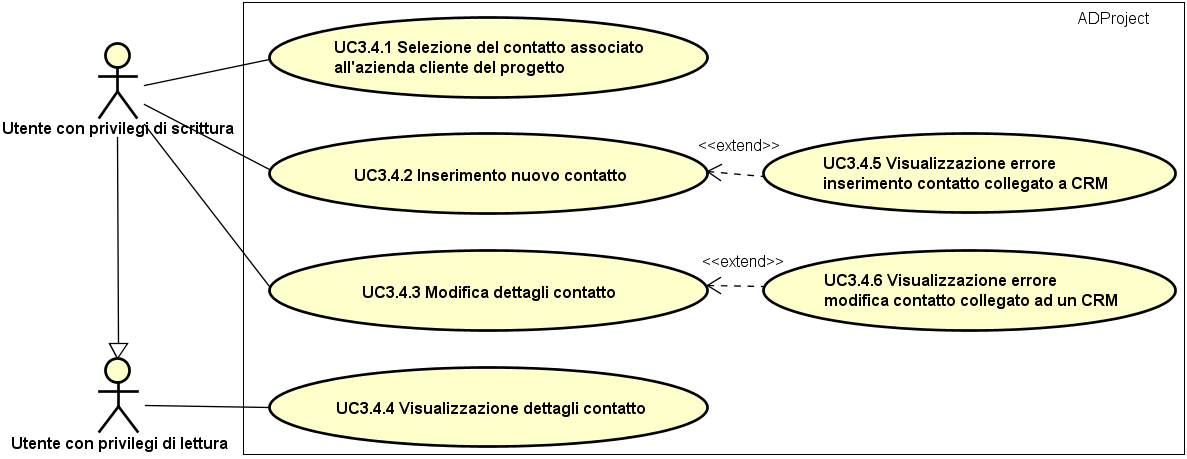
\includegraphics[scale=0.5]{images/useCase/UC3_4}
		\caption{Use Case 3.4 - Gestione contatto principale}
		%\caption{}
		\label{fig:uc3.4}
	\end{figure}
	\begin{longtable}{ | p{2.7cm} | p{12cm} |}
		\hline \textbf{Attori} & Utente con privilegi di scrittura\\ 
		\hline \textbf{Descrizione} & Attraverso l’interfaccia di configurazione di progetto, l’utente coi permessi corretti è in grado di modificare le informazioni relative al contatto principale di riferimento per un progetto (il PM lato cliente)\\ 
		\hline \textbf{Scenario Principale} & \begin{enumerate}
			\itemsep-0.5em 
			\item L’utente seleziona uno dei contatti associato al cliente selezionato per il progetto  (UC3.4.1);
			\item L’utente inserisce un nuovo contatto  (UC3.4.2);
			\item L’utente modifica i dettagli relativi al contatto di riferimento per il progetto  (UC3.4.3);
			\item L’utente visualizza i dettagli relativi al contatto inserito  (UC3.4.4).
			
		\end{enumerate}
		\\ 
		\hline \textbf{Estensioni} & \begin{enumerate}
			\item Viene visualizzato un messaggio d'errore se si tenta di aggiungere un contatto principale prima che sia associato un'azienda cliente al progetto (UC3.12);
			
		\end{enumerate}
		\\ 
		\hline \textbf{Postcondizione} & Sono state modificate le informazioni relative al contatto principale di riferimento per un progetto \\ 
		\hline 
	\end{longtable}
	
	\hypertarget{UC3.5}{}
	\subsection{Caso d'uso UC3.5: Creazione nuovo progetto da offerta}
		\begin{figure}[H]
		\centering
		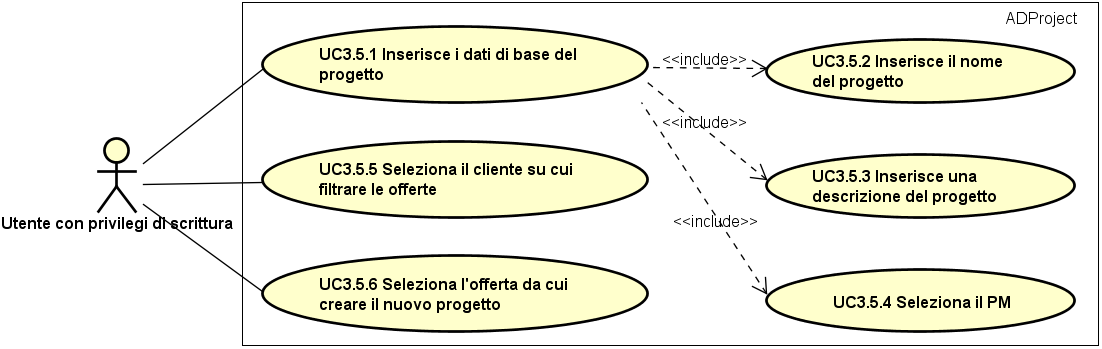
\includegraphics[scale=0.55]{images/useCase/UC3_5}
		\caption{Use Case 3.5 - Creazione progetto da offerta}
		%\caption{}
		\label{fig:uc3.5}
	\end{figure}
	\begin{longtable}{ | p{2.7cm} | p{12cm} |}
		\hline \textbf{Attori} & Utente con privilegi di scrittura\\ 
		\hline \textbf{Descrizione} & L'utente crea un progetto a partire dai dati di una specifica offerta, auto-completando quindi l'associazione tra progetto con account, offerta e contatto\\ 
		\hline \textbf{Scenario Principale} & \begin{enumerate}
			\itemsep-0.5em 
			\item L’utente inserisce i dati di base del progetto  (UC3.5.1);
			\item L’utente selezione il cliente su cui filtrare le offerte  (UC3.5.2);
			\item L’utente seleziona l’offerta da cui creare il nuovo progetto  (UC3.5.3).
			
		\end{enumerate}
		\\ 
		\hline \textbf{Postcondizione} & Viene creato un nuovo progetto\\ 
		\hline 
	\end{longtable}